% Options for packages loaded elsewhere
\PassOptionsToPackage{unicode}{hyperref}
\PassOptionsToPackage{hyphens}{url}
\PassOptionsToPackage{dvipsnames,svgnames,x11names}{xcolor}
%
\documentclass[
  letterpaper,
  DIV=11,
  numbers=noendperiod]{scrreprt}

\usepackage{amsmath,amssymb}
\usepackage{iftex}
\ifPDFTeX
  \usepackage[T1]{fontenc}
  \usepackage[utf8]{inputenc}
  \usepackage{textcomp} % provide euro and other symbols
\else % if luatex or xetex
  \usepackage{unicode-math}
  \defaultfontfeatures{Scale=MatchLowercase}
  \defaultfontfeatures[\rmfamily]{Ligatures=TeX,Scale=1}
\fi
\usepackage{lmodern}
\ifPDFTeX\else  
    % xetex/luatex font selection
\fi
% Use upquote if available, for straight quotes in verbatim environments
\IfFileExists{upquote.sty}{\usepackage{upquote}}{}
\IfFileExists{microtype.sty}{% use microtype if available
  \usepackage[]{microtype}
  \UseMicrotypeSet[protrusion]{basicmath} % disable protrusion for tt fonts
}{}
\makeatletter
\@ifundefined{KOMAClassName}{% if non-KOMA class
  \IfFileExists{parskip.sty}{%
    \usepackage{parskip}
  }{% else
    \setlength{\parindent}{0pt}
    \setlength{\parskip}{6pt plus 2pt minus 1pt}}
}{% if KOMA class
  \KOMAoptions{parskip=half}}
\makeatother
\usepackage{xcolor}
\setlength{\emergencystretch}{3em} % prevent overfull lines
\setcounter{secnumdepth}{5}
% Make \paragraph and \subparagraph free-standing
\ifx\paragraph\undefined\else
  \let\oldparagraph\paragraph
  \renewcommand{\paragraph}[1]{\oldparagraph{#1}\mbox{}}
\fi
\ifx\subparagraph\undefined\else
  \let\oldsubparagraph\subparagraph
  \renewcommand{\subparagraph}[1]{\oldsubparagraph{#1}\mbox{}}
\fi


\providecommand{\tightlist}{%
  \setlength{\itemsep}{0pt}\setlength{\parskip}{0pt}}\usepackage{longtable,booktabs,array}
\usepackage{calc} % for calculating minipage widths
% Correct order of tables after \paragraph or \subparagraph
\usepackage{etoolbox}
\makeatletter
\patchcmd\longtable{\par}{\if@noskipsec\mbox{}\fi\par}{}{}
\makeatother
% Allow footnotes in longtable head/foot
\IfFileExists{footnotehyper.sty}{\usepackage{footnotehyper}}{\usepackage{footnote}}
\makesavenoteenv{longtable}
\usepackage{graphicx}
\makeatletter
\def\maxwidth{\ifdim\Gin@nat@width>\linewidth\linewidth\else\Gin@nat@width\fi}
\def\maxheight{\ifdim\Gin@nat@height>\textheight\textheight\else\Gin@nat@height\fi}
\makeatother
% Scale images if necessary, so that they will not overflow the page
% margins by default, and it is still possible to overwrite the defaults
% using explicit options in \includegraphics[width, height, ...]{}
\setkeys{Gin}{width=\maxwidth,height=\maxheight,keepaspectratio}
% Set default figure placement to htbp
\makeatletter
\def\fps@figure{htbp}
\makeatother

\usepackage{pdfpages}
\KOMAoption{captions}{tableheading}
\makeatletter
\@ifpackageloaded{tcolorbox}{}{\usepackage[skins,breakable]{tcolorbox}}
\@ifpackageloaded{fontawesome5}{}{\usepackage{fontawesome5}}
\definecolor{quarto-callout-color}{HTML}{909090}
\definecolor{quarto-callout-note-color}{HTML}{0758E5}
\definecolor{quarto-callout-important-color}{HTML}{CC1914}
\definecolor{quarto-callout-warning-color}{HTML}{EB9113}
\definecolor{quarto-callout-tip-color}{HTML}{00A047}
\definecolor{quarto-callout-caution-color}{HTML}{FC5300}
\definecolor{quarto-callout-color-frame}{HTML}{acacac}
\definecolor{quarto-callout-note-color-frame}{HTML}{4582ec}
\definecolor{quarto-callout-important-color-frame}{HTML}{d9534f}
\definecolor{quarto-callout-warning-color-frame}{HTML}{f0ad4e}
\definecolor{quarto-callout-tip-color-frame}{HTML}{02b875}
\definecolor{quarto-callout-caution-color-frame}{HTML}{fd7e14}
\makeatother
\makeatletter
\@ifpackageloaded{bookmark}{}{\usepackage{bookmark}}
\makeatother
\makeatletter
\@ifpackageloaded{caption}{}{\usepackage{caption}}
\AtBeginDocument{%
\ifdefined\contentsname
  \renewcommand*\contentsname{Table of contents}
\else
  \newcommand\contentsname{Table of contents}
\fi
\ifdefined\listfigurename
  \renewcommand*\listfigurename{List of Figures}
\else
  \newcommand\listfigurename{List of Figures}
\fi
\ifdefined\listtablename
  \renewcommand*\listtablename{List of Tables}
\else
  \newcommand\listtablename{List of Tables}
\fi
\ifdefined\figurename
  \renewcommand*\figurename{Figure}
\else
  \newcommand\figurename{Figure}
\fi
\ifdefined\tablename
  \renewcommand*\tablename{Table}
\else
  \newcommand\tablename{Table}
\fi
}
\@ifpackageloaded{float}{}{\usepackage{float}}
\floatstyle{ruled}
\@ifundefined{c@chapter}{\newfloat{codelisting}{h}{lop}}{\newfloat{codelisting}{h}{lop}[chapter]}
\floatname{codelisting}{Listing}
\newcommand*\listoflistings{\listof{codelisting}{List of Listings}}
\makeatother
\makeatletter
\makeatother
\makeatletter
\@ifpackageloaded{caption}{}{\usepackage{caption}}
\@ifpackageloaded{subcaption}{}{\usepackage{subcaption}}
\makeatother
\ifLuaTeX
  \usepackage{selnolig}  % disable illegal ligatures
\fi
\usepackage{bookmark}

\IfFileExists{xurl.sty}{\usepackage{xurl}}{} % add URL line breaks if available
\urlstyle{same} % disable monospaced font for URLs
\hypersetup{
  pdftitle={PTR Portfolio},
  pdfauthor={Eric M Reyes},
  colorlinks=true,
  linkcolor={blue},
  filecolor={Maroon},
  citecolor={Blue},
  urlcolor={Blue},
  pdfcreator={LaTeX via pandoc}}

\title{PTR Portfolio}
\author{Eric M Reyes}
\date{Submitted: September 2024}

\begin{document}
\maketitle

\renewcommand*\contentsname{Table of contents}
{
\hypersetup{linkcolor=}
\setcounter{tocdepth}{2}
\tableofcontents
}
\bookmarksetup{startatroot}

\chapter*{Note to the Reader}\label{note-to-the-reader}
\addcontentsline{toc}{chapter}{Note to the Reader}

\markboth{Note to the Reader}{Note to the Reader}

\begin{quote}
Certain authors, speaking of their works, say ``My book,'' ``My
commentary,'' ``My history,'' etc\ldots.They would do better to say
``Our book,'' ``Our commentary,'' ``Our history,'' etc., because there
is in them usually more of other people's than their own.
(Pascal)\footnote{\href{https://www.gutenberg.org/files/18269/18269-h/18269-h.htm\#p_43}{Pascal,
  Blaise. \emph{Pascal's Penées}. (1958) New York:EP Dutton, (\#43)}}
\end{quote}

At the peak of summer, as a heat wave enveloped the country, the horn
blast signaled the start of the Mac --- the longest annual freshwater
sailing race in the world where hundreds of sailors gather to race
across Lake Michigan and Lake Huron from Chicago to Mackinac Island.
Wanting to witness the magic, we maneuvered the boat to the outside of
the fleet and watched as teams capitalized on the southerly winds,
dotting the horizon with spinnakers\footnote{a large sail that acts as a
  kite, allowing the wind to push the boat downwind
  (\href{https://drive.google.com/file/d/1NrW5GJNlNJxoZi73NggF7sHlc6oJlpdx/view?usp=sharing}{seen
  here in an image from the 2024 race start}).}. In that moment, as I
stood at the helm, the boat and wind gently rocking our ship, I was at
peace knowing there was no where else I wanted to be.

While I have no aspirations of ever competing in the Mac, I have enjoyed
learning to sail over the past several years. Each summer day on the
water harnessing the wind (with no particular destination in mind)
soothes the wounds of a hard academic year. And, each outing provides a
learning opportunity --- a chance for my boat to teach me a bit more
about being a sailor. Early this summer, my youngest daughter asked if I
would take her out, ``just the two of us,'' for the afternoon and teach
her more about sailing. Including her in the preparations, she tied
knots and steered our course as I raised the sails. Just as we got
underway, the wind caught my hat and sent it flying into the lake. The
outing was now a lesson in conducting a crew-over-board maneuver (it was
a nice hat). The standard maneuver required that we sail away from the
hat, turn through the wind, and then approach the hat from downwind so
that we could easily control our speed --- me steering a steady course
allowing my daughter to reach overboard and retrieve the hat.

To an onlooker only familiar with powered vessels, my actions would seem
strange. Instead of turning immediately to recover the hat, we chose to
first sail farther away. An abrupt turn easily executed on a powered
vessel could result in the sailboat capsizing. In that moment, success
required that I employ my knowledge and skills not only to achieving my
personal desires (I wanted that hat back) but also to safeguarding the
well-being of the vessel and its crew. I believe the same should be true
within academia. The success/strength of a portfolio should not be
determined solely by the line items on a faculty member's CV; we should
also consider how the faculty member has stewarded the mission of the
Institute to its benefit, including its faculty and students.

This portfolio reflects on the decisions I have made in charting the
course of my career. While I am uncertain of my destination, I can
describe my current direction and the principles that guide that
direction. As such, this portfolio is organized around the facets of my
professional mission and vision, developed alongside a group of
colleagues\footnote{During the 2021-2022 academic year, supported by the
  Center for the Practice of Scholarship and Education, I facilitated a
  reading of Susan Robison's
  \href{http://peakperformingprofessor.com/ppp/}{\emph{The Peak
  Performing Professor: A Practical Guide to Productivity and
  Happiness}} with five colleagues. I owe a great deal to the
  conversations with these amazing women: Eva Andrijcic, Sylvia
  Carlisle, Heather Chenette, Michelle Marincel Payne, and Jenny
  Mueller.}, that guide my professional activities. I routinely tell my
students they should never trust a study that omits a ``limitations''
section; as such, this portfolio reflects on both my positive intent and
areas of concern. I then submit to your determination whether my path is
of benefit to the Institute.

\begin{tcolorbox}[enhanced jigsaw, breakable, toptitle=1mm, arc=.35mm, leftrule=.75mm, bottomrule=.15mm, titlerule=0mm, opacitybacktitle=0.6, colbacktitle=quarto-callout-note-color!10!white, opacityback=0, colframe=quarto-callout-note-color-frame, toprule=.15mm, left=2mm, bottomtitle=1mm, coltitle=black, colback=white, title=\textcolor{quarto-callout-note-color}{\faInfo}\hspace{0.5em}{Note}, rightrule=.15mm]

This portfolio was designed to be read online
(\href{https://reyesem.github.io/Full-Professor-Packet/}{click here}).
However, the PDF version retains all required content.

\end{tcolorbox}

\bookmarksetup{startatroot}

\chapter{A Teacher, but Not an
Educator}\label{a-teacher-but-not-an-educator}

\begin{quote}
Teachers can fan flames that are already there, but usually cannot
create the spark that first attracts a person to something\ldots There
is no accounting for desire. Who knows why we are drawn to the things
that attract us. Teachers exist to serve such attractions, not create
them; otherwise we are no longer teacher{[}s{]} but evangelists.
(Sells)\footnote{\href{https://www.amazon.com/Soul-Sailing-Benjamin-Sells/dp/1710340894}{Sells,
  Ben. \emph{The Soul of Sailing}. (2019)}}
\end{quote}

\begin{quote}
Assigning grades was the easy way out of doing the ``actual work'' of
teaching\ldots When I eliminated grades it tested my creativity and
patience. I was forced to rethink what went on in my class.
(Blackwelder)\footnote{\href{https://wvupressonline.com/ungrading}{Aaron
  Blackwelder in \emph{Ungrading: Why Rating Students Undermines
  Learning (and what to Do Instead)} (2020), edited by Susan Blum.}}
\end{quote}

These two quotes, side by side, capture the battle that has waged within
me over the years as I have navigated my role in the classroom. Like
Blackwelder, the idealist in me believes in connecting with others and
inspiring them to learn; however, the realist in me resonates with
Sells, accepting that I cannot manifest in someone the same joy in the
material I have. In an attempt to reconcile these ideas, we might
distinguish between a teacher and an educator.

\begin{tcolorbox}[enhanced jigsaw, breakable, toptitle=1mm, arc=.35mm, leftrule=.75mm, bottomrule=.15mm, titlerule=0mm, opacitybacktitle=0.6, colbacktitle=quarto-callout-tip-color!10!white, opacityback=0, colframe=quarto-callout-tip-color-frame, toprule=.15mm, left=2mm, bottomtitle=1mm, coltitle=black, colback=white, title=\textcolor{quarto-callout-tip-color}{\faLightbulb}\hspace{0.5em}{Educator vs.~Teacher}, rightrule=.15mm]

A teacher provides instruction, guidance, and feedback during the
learning process. In contrast, an educator goes beyond teaching,
inspiring students toward an interest and passion in the material.

\end{tcolorbox}

My growth as a teacher has coincided with a decrease in my student
course evaluations. Understanding that these evaluations primarily
reflect the student experience, I believe this trend reveals that I have
struggle more and more to connect with my students, making it difficult
to inspire them. As a result, I am not the educator I aspire to be;
however, I have leaned into what I view as my primary responsibility as
a teacher: providing rich learning opportunities.

\begin{tcolorbox}[enhanced jigsaw, breakable, toptitle=1mm, arc=.35mm, leftrule=.75mm, bottomrule=.15mm, titlerule=0mm, opacitybacktitle=0.6, colbacktitle=quarto-callout-important-color!10!white, opacityback=0, colframe=quarto-callout-important-color-frame, toprule=.15mm, left=2mm, bottomtitle=1mm, coltitle=black, colback=white, title=\textcolor{quarto-callout-important-color}{\faExclamation}\hspace{0.5em}{My Professional Mission as a Teacher}, rightrule=.15mm]

To \emph{design high quality learning experiences} for students who want
to use data with integrity and educators who want to impact students.

\end{tcolorbox}

During the Fall of 2020, my grandmother was losing her battle with
cancer. With the COVID pandemic at its height, my courses had
transitioned to a hybrid delivery meeting twice weekly, and I leveraged
this to be with my grandmother during her final days. I would lead four
sections of my Introductory course, then drive North of Indianapolis to
spend time with family and help where I could, shifting between helping
make a meal and meeting with students on Teams. Forty-eight hours later,
I would return to Terre Haute for the next class meeting. The
flexibility that had been built into my course allowed me to be present
with students and my family in a way that I would not have previously
thought possible. I place high importance on designing learning
experiences that are flexible.

\begin{tcolorbox}[enhanced jigsaw, breakable, toptitle=1mm, arc=.35mm, leftrule=.75mm, bottomrule=.15mm, titlerule=0mm, opacitybacktitle=0.6, colbacktitle=quarto-callout-tip-color!10!white, opacityback=0, colframe=quarto-callout-tip-color-frame, toprule=.15mm, left=2mm, bottomtitle=1mm, coltitle=black, colback=white, title=\textcolor{quarto-callout-tip-color}{\faLightbulb}\hspace{0.5em}{Flexibility in Course Design}, rightrule=.15mm]

Students benefit from structure in a course, but designing those
structures to be flexible allows learning to take place in the midst of
external shocks to the life of the professor and/or students.

\end{tcolorbox}

Since the pandemic, I have transitioned the vast majority of my courses
to a hybrid structure to promote flexibility for my students (and
myself) and allow me to operate out of my strengths. But, this
transition has required that I commit time to creating resources to
promote student success in this environment. For example, I converted my
lecture notes to online texts.\footnote{I have a text for each course I
  teach regularly, including
  \href{https://reyesem.github.io/introstat-text/}{MA223 Introductory
  Statistics}, \href{https://reyesem.github.io/biostat-text/}{MA482
  Biostatistics}, and \href{https://reyesem.github.io/bayes-text/}{MA483
  Bayesian Statistics}. I revise the materials and continue to develop
  new material as my courses develop.} Available online (and for
download as a PDF), the design of this portfolio mimics the design of
the texts available to students. In addition to a text, my courses
include videos covering key concepts and examples (see
Figure~\ref{fig-confounding-video} for an example); and, note packets
guide students through the resources and encourage them to take a more
active role in summarizing content.

\begin{figure}

\centering{

\href{https://rose-hulman.hosted.panopto.com/Panopto/Pages/Viewer.aspx?id=2bb062ec-399b-43dd-b188-b1af016191f1}{\includegraphics{img-concept-clip.jpg}}

}

\caption{\label{fig-confounding-video}Example ``concept clip'' used in
my Introductory Statistics course to discuss confounding.}

\end{figure}%

\begin{tcolorbox}[enhanced jigsaw, breakable, toptitle=1mm, arc=.35mm, leftrule=.75mm, bottomrule=.15mm, titlerule=0mm, opacitybacktitle=0.6, colbacktitle=quarto-callout-note-color!10!white, opacityback=0, colframe=quarto-callout-note-color-frame, toprule=.15mm, left=2mm, bottomtitle=1mm, coltitle=black, colback=white, title=\textcolor{quarto-callout-note-color}{\faInfo}\hspace{0.5em}{Importance of Moodle}, rightrule=.15mm]

Moodle plays an integral part of my course design, and it is an
extension of my classroom (or maybe, the classroom is an extension of my
Moodle course). A visit to my class would not tell you nearly as much
about my teaching philosophy as my Moodle course. For those interested,
I have an example course available to peruse by
\href{https://moodle.rose-hulman.edu/course/view.php?id=104992}{clicking
here}.

\end{tcolorbox}

A course calendar provides guidance on pacing through the material
between class meetings, but the resources are available for students to
review as their schedule permits.

\begin{quote}
One strength of the course is the flipped classroom. Being able to watch
the lecture videos whenever I needed them helped me learn the content at
my pace, and review the content when I did not fully grasp the topic.
(MA223 student)
\end{quote}

\begin{tcolorbox}[enhanced jigsaw, breakable, toptitle=1mm, arc=.35mm, leftrule=.75mm, bottomrule=.15mm, titlerule=0mm, opacitybacktitle=0.6, colbacktitle=quarto-callout-note-color!10!white, opacityback=0, colframe=quarto-callout-note-color-frame, toprule=.15mm, left=2mm, bottomtitle=1mm, coltitle=black, colback=white, title=\textcolor{quarto-callout-note-color}{\faInfo}\hspace{0.5em}{MA223 Introductory Statistics}, rightrule=.15mm]

Named ``Engineering Statistics I,''
\href{https://reyesem.github.io/ma223sample.html}{MA223} is the
introductory statistics course required by most science and engineering
programs on campus. The course emphasizes statistical literacy (speaking
the language of statistics and interpreting statistical methods and
results), reasoning (defining the need for data to address questions,
understanding the role and impact of variability), design (approaches to
data collection and the impact of the study design on the conclusions),
and analysis (choosing an appropriate methodology and using a
statistical computing environment to carry out an analysis). The
concepts are introduced in the context of science and engineering
applications.

\end{tcolorbox}

Primary content delivery happens remotely. In-class meetings are
reserved for topics that would benefit from discussions or additional
examples, attempting to take more abstract concepts and make them
tangible. I broadcast these discussions on Teams so that students can
engage remotely if they are unable to attend in person. To provide
flexibility during assessments, I have transitioned to take-home exams
and emphasize projects, often allowing students to collaborate. This
also facilitates my transition to alternative grading schemes, which
relies on students revising work.

\begin{quote}
The revision system really assisted with my learning, along with the
resources the professor provided. Although the course was difficult, the
course structure allowed for me to learn material quicker and more
effectively. (MA483 student)
\end{quote}

\begin{tcolorbox}[enhanced jigsaw, breakable, toptitle=1mm, arc=.35mm, leftrule=.75mm, bottomrule=.15mm, titlerule=0mm, opacitybacktitle=0.6, colbacktitle=quarto-callout-note-color!10!white, opacityback=0, colframe=quarto-callout-note-color-frame, toprule=.15mm, left=2mm, bottomtitle=1mm, coltitle=black, colback=white, title=\textcolor{quarto-callout-note-color}{\faInfo}\hspace{0.5em}{MA483 Bayesian Data Analysis}, rightrule=.15mm]

An interesting course in the curriculum,
\href{https://reyesem.github.io/ma483sample.html}{MA483} provides a
different framework for conducting statistical inference. It acts as
both an upper-level elective for those who are specializing in
statistics as well as an alternate introductory course for those in
disciplines that require only probability (such as computer science and
electrical engineering).

\end{tcolorbox}

The asynchronous days are not ``days off.'' In order to meet deadlines,
students are expected to engage with material daily, as outlined in the
course calendar. Asynchronous days also provide ample opportunity for me
to meet with students to address questions over assignments. While some
students prefer in-person meetings, I have a growing number that prefer
engaging remotely. For some students, they enjoy the convenience of
reaching out from their residence hall (or academic space) without
needing to pack up and trek to my office. Others take advantage of
receiving help when they are feeling ill.~I enjoy being able to have
students share their screen when debugging code. I also have noticed an
increase in the number of students who prefer to correspond over Teams
messages, sharing screen shots of work as necessary; I find this
benefits students who are internal processors. It removes that
additional, and unnecessary, anxiety that accompanies a feeling of
needing to respond to my prompts immediately; instead, they take the
time they need.

\begin{quote}
Dr.~Reyes was always helpful and available outside of class which was
much appreciated. (MA386 student)
\end{quote}

\begin{tcolorbox}[enhanced jigsaw, breakable, toptitle=1mm, arc=.35mm, leftrule=.75mm, bottomrule=.15mm, titlerule=0mm, opacitybacktitle=0.6, colbacktitle=quarto-callout-note-color!10!white, opacityback=0, colframe=quarto-callout-note-color-frame, toprule=.15mm, left=2mm, bottomtitle=1mm, coltitle=black, colback=white, title=\textcolor{quarto-callout-note-color}{\faInfo}\hspace{0.5em}{MA386 Statistical Programming}, rightrule=.15mm]

\href{https://reyesem.github.io/ma386sample.html}{MA386} introduces
students to the computational tools and skills necessary to operate at
all stages of the ``analysis pipeline.'' This course is popular among
students seeking a minor in Data Science as well as those in the
biological sciences, as it prepares them for working with data in their
own projects.

\end{tcolorbox}

Each of these decisions regarding my course design has been in the
pursuit of courses that add flexibility --- flexibility that I hope
removes the stress to perform in the midst of other demands and gives
students space to enjoy the learning.

\begin{quote}
This is, by far, one of my favorite classes that I have ever taken at
Rose. Dr.~Reyes was definitely a large part in this class being so
enjoyable - his teaching methods, avaibility for offering help, and
general attitude made me feel excited to be engaged in the
class\ldots Course policies were clearly oriented to help me learn more
than anything else. (MA482 student)
\end{quote}

\begin{tcolorbox}[enhanced jigsaw, breakable, toptitle=1mm, arc=.35mm, leftrule=.75mm, bottomrule=.15mm, titlerule=0mm, opacitybacktitle=0.6, colbacktitle=quarto-callout-note-color!10!white, opacityback=0, colframe=quarto-callout-note-color-frame, toprule=.15mm, left=2mm, bottomtitle=1mm, coltitle=black, colback=white, title=\textcolor{quarto-callout-note-color}{\faInfo}\hspace{0.5em}{MA482 Biostatistics}, rightrule=.15mm]

The biological sciences often yield data that present unique challenges
to analysis. A second course in statistics,
\href{https://reyesem.github.io/ma482sample.html}{MA482} introduces
these challenges and the statistical methods employed to overcome them.

\end{tcolorbox}

My course design was influenced heavily by
\href{https://udlguidelines.cast.org/}{universal design for learning}
concepts, especially trying to promote accessibility. My syllabi include
an infographic cover page that summarizes key policies; un-timed
take-home assessments have eliminated testing accommodations; and, video
lectures with captions allow students to take in the material at their
pace. While I believe all students benefit from these policies, they do
require discipline on the part of the student, and not all students
respond well to the structure. The primary concern I hear is that
students believe they are ``teaching themselves'' because I do not
lecture regularly in class. This is particularly true in the
introductory course.

\begin{quote}
I felt like I was teaching myself this course and had to put so much
effort into just figuring out what I'm missing. (MA223 student)
\end{quote}

\begin{quote}
The learning in the class is reliant heavily on the student. (MA223
student)
\end{quote}

I design the learning opportunities, but I do not force the students to
engage with them, and as a result, I admit that I do lose some students.
Yet, I stick with this structure because it allows me to operate out of
my strengths. I deliver good lectures, but I do not think I resonate
best with students in that format. Especially over the past few years, I
have found it challenging to connect with students broadly. Examples
from their discipline; stories from those in industry; personal
experience; topics in social justice; even self-deprecating
humor\ldots these tactics that once drew students in are failing me. As
a result, my lectures only reach those who are intrinsically motivated
--- a small percentage of students. Transitioning away from lecture
being at the forefront allows my class to rely heavily on multimedia,
tutorials, and assignments crafted to encourage questions. And, I think
I am better at constructing these resources than constructing lectures.
My course structure provides time for me to engage with students on
these assignments through a variety of media that I am very comfortable
in (whether in person or on Teams messages, emails, etc.) and allows for
ample time to give feedback on those assignments. This feedback is
integral to the alternative grading structures that are fundamental to
how learning takes place in my courses.

\begin{quote}
Even though I might have not gotten full credit on an assignment the
first time, I was allowed to go back and read the feedback of where I
went wrong, and resumbit again for full credit. I very much perfer this
class structure because it actually encourages learning through
mistakes\ldots{} (MA223 student)
\end{quote}

Essentially, I believe this structure capitalizes on my strengths as a
\emph{teacher} and minimizes the impacts of my struggles as an
\emph{educator}. One shortcoming that my approach has highlighted is my
compulsion to ``reinvent the wheel.'' In putting together resources for
my students, I create things from scratch. I rarely rely on published
texts or existing videos. I prefer to control the narrative, and that
does take time. I have at times overcome my own ego in this regard; due
to the speed at which the content changes, I rely on existing resources
for MA386 Statistical Programming. However, I review and update the
resources each time I teach the course.

As I consider my path, I would like to improve on how I advise senior
capstone experiences. Some of my previous experiences have been amazing,
but many more have fallen short of my expectations. In these instances,
I have both failed to motivate the student to the benefits of these
capstones and to provide the structure necessary to help them succeed
(erring on the side of too much flexibility). For the past few months, I
have worked with Megan Heyman on redesigning the senior capstone
experience for students interested in Statistics. Fall 2024 will be our
first time implementing the new structure; however, having approached
this as a course design, and with Megan's strengths in adding structure,
I am already certain it will be an improvement.

During the summer of 2020, the Institute recognized the need for a
coordinated response to teaching during the pandemic, both through
delivering course content in alternate formats but also training faculty
to design courses that leverage these modalities. Having taught online
and served as our department's Moodle mentor for a number of years, I
was thrilled when Kay C Dee and Ella Ingram asked me to be a mentor for
the Creating Adaptable Courses curriculum and the Y1 course creation
efforts heading into the 2020-2021 academic year. We believed in this
training effort so much that a group of us authored a book chapter
(appearing in
\href{https://uen.pressbooks.pub/resilientpedagogy/}{\emph{Resilient
Pedagogy: Practical Teaching Strategies to Overcome Distance,
Disruption, and Distraction}}) describing the curriculum for other
course designers.

Being a part of the Creating Adaptable Courses curriculum also reminded
me how much I enjoy supporting faculty course development. Over the
following summers, I became more involved in the Fall Teaching Workshop
for incoming faculty. At Ella's invitation, I led a session on backward
design during the 2021 Workshop, and I have co-organized the 2022 (with
Ella Ingram), 2023 (with Rich House), and 2024 (with Rich House and
Aimee Cloutier) workshops. My largest contribution to the workshop has
been working with Kay C Dee to transform the ``Introduction to Moodle''
session into an opportunity for new faculty to begin developing their
course Moodle pages alongside senior faculty with whom they will be
co-teaching. This experience can be rewarding to both incoming faculty
(grateful to begin course prep) and senior faculty (integrating fresh
perspectives of the new faculty). This is an example of where the
\emph{design}, not the implementation, is where I have had an impact.
During the session, I answer a few questions, but I mostly just watch
the magic happen.

\begin{tcolorbox}[enhanced jigsaw, breakable, toptitle=1mm, arc=.35mm, leftrule=.75mm, bottomrule=.15mm, titlerule=0mm, opacitybacktitle=0.6, colbacktitle=quarto-callout-tip-color!10!white, opacityback=0, colframe=quarto-callout-tip-color-frame, toprule=.15mm, left=2mm, bottomtitle=1mm, coltitle=black, colback=white, title=\textcolor{quarto-callout-tip-color}{\faLightbulb}\hspace{0.5em}{Operating from My Strengths}, rightrule=.15mm]

While I have struggled to motivate students, I am at my best when
designing the course. Those designs play to my strengths in remote
engagement, but they are driven by flexibility.

\end{tcolorbox}

\bookmarksetup{startatroot}

\chapter{Being Infected by the Curiosity of
Others}\label{being-infected-by-the-curiosity-of-others}

\begin{quote}
I'll work hard I'll do my part; You won't hear me complain; I'll never
go down easy; I swear I'll pull my weight. (Sawyer Brown)\footnote{From
  \emph{The Nebraska Song} by \href{https://sawyerbrown.com/}{Sawyer
  Brown}. As I am sure my Department Head and others will attest, I am
  still working on the ``not complaining'' part!}
\end{quote}

I attended graduate school intent on entering industry; the primary
reason I did not initially consider academia was my aversion to
``research.'' In general, I have struggled to find the drive required to
plan and execute an agenda from idea through publication. Two examples
illustrate this. Suppose we are interested in determining which
characteristics recorded in a patient's medical chart (potential
predictors) are associated with experiencing a heart attack (the
response); however, we might only have the patient's family history for
a subset of the study participants. Separating the characteristics
associated with a response from those that are not is a process known as
variable selection; and, as described in our example, we might be
interested in doing this in the presence of missing data. For a number
of years, I have nursed an idea of a general approach to this problem
that merges techniques developed concurrently in separate areas of
statistics. Several years ago, I even advised a senior capstone (Cody
Roberts, 2015) in this area with promising results. However, I have not
pursued the project, continuing instead to prioritize revisions to class
materials or the development of new courses (or really any other work).
During the 2022-2023 academic year, upon advice from a colleague, I
reviewed the literature on how alternative grading can improve equity in
the classroom. A student (Clara Place, expected 2025) helped me conduct
a survey to better understand the experiences of historically
underrepresented students with alternative grading at Rose-Hulman. I
completed the paper, but it was rejected from the target journal; and,
it has just sat since, me prioritizing day-to-day work.

While I have not developed a research agenda, I have remained active. We
should expect faculty to continue to grow intellectually; for me, this
growth is fueled by the curiosity of others. The most appealing aspect
of Statistics for me has always been the ability to collaborate with
researchers across a variety of disciplines. As an applied statistician,
my passion is joining such collaborations, particularly in the
biological sciences. The development of an appropriate analysis plan,
the implementation of the analysis, and the communication of the
results, all in the service of advancing the research being led by
others is where I perform best. These opportunities invigorate me,
enrich my classroom, have meaningful impacts, and contribute to my
growth as a scholar.

\begin{tcolorbox}[enhanced jigsaw, breakable, toptitle=1mm, arc=.35mm, leftrule=.75mm, bottomrule=.15mm, titlerule=0mm, opacitybacktitle=0.6, colbacktitle=quarto-callout-important-color!10!white, opacityback=0, colframe=quarto-callout-important-color-frame, toprule=.15mm, left=2mm, bottomtitle=1mm, coltitle=black, colback=white, title=\textcolor{quarto-callout-important-color}{\faExclamation}\hspace{0.5em}{My Professional Mission as a Collaborator}, rightrule=.15mm]

To \emph{collaborate} with researchers who want to make a difference.

\end{tcolorbox}

\begin{tcolorbox}[enhanced jigsaw, breakable, toptitle=1mm, arc=.35mm, leftrule=.75mm, bottomrule=.15mm, titlerule=0mm, opacitybacktitle=0.6, colbacktitle=quarto-callout-note-color!10!white, opacityback=0, colframe=quarto-callout-note-color-frame, toprule=.15mm, left=2mm, bottomtitle=1mm, coltitle=black, colback=white, title=\textcolor{quarto-callout-note-color}{\faInfo}\hspace{0.5em}{Note}, rightrule=.15mm]

As I am both a statistician and a professor, and my collaborations over
the years have resulted in growth in both realms.

\end{tcolorbox}

I am a huge proponent of alternative grading strategies\footnote{I have
  documented several of my experiences on my
  \href{https://reyesem.github.io/specsgrading.html}{personal site} in
  hopes of benefiting others.} and could talk about them for
hours\footnote{On a recent road trip, my wife, an adjunct in our
  department, and I spent 8+ hours talking about grading!}. Over the
past several years, I have engaged in several opportunities to share my
experience with others. This has included two workshops for Rose-Hulman
faculty (the first co-led with John Mirth, the second co-led with Sylvia
Carlisle), two invited contributions to the
\href{https://stattlc.com/2021/02/04/specifications-grading-an-overview/}{Statistics
Teaching and Learning Corner}, a conference presentation with several
Rose-Hulman colleagues (Emma Dosmar, Julia Williams, Rich House, and
Sylvia Carlisle), and a wonderful collaboration with educators from
several universities (Brenna Curley of Moravian University, Jillian
Downey of Gustavus Adolphus College, Katherine M. Kinnaird of U.S. Air
Force Academy and Smith College, and Adam Loy of Carleton College). This
latest collaboration has resulted in a publication in the
\href{https://www.tandfonline.com/doi/full/10.1080/26939169.2023.2277851}{\emph{Journal
for Statistics and Data Science Education}} and a workshop at the
\href{https://www.causeweb.org/cause/uscots/uscots23/w14-communicating-progress-statistics-course-through-non-traditional-grading-room}{US
Conference on Teaching Statistics}.

Through each of these experiences, the colleagues I have worked with
have helped me refine my approach to grading. In fact, the regular
meetings with my latest collaborators have become a high point in my
schedule, providing a source of energy for tackling the difficult parts
of teaching. These conversations have been so fruitful and so cathartic
to each of us that our latest venture is launching a podcast for
educators where we ``talk through teaching tensions together'' in an
effort to share the various experiences educators have in tackling daily
challenges in education like navigating the use of technology in the
classroom. It was a great joy to see our hard work recognized in the
acceptance of our paper; but, the greater joy (being the ``senior''
member of the group) was watching all four of my colleagues receive
positive tenure decisions following its acceptance.

In addition to my position at Rose-Hulman, I hold the position of
Adjunct Clinical Assistant Professor of Biostatistics \& Health Data
Science through Indiana University. This position supports my work with
the Terre Haute branch of the Indiana University School of Medicine,
which houses the
\href{https://medicine.iu.edu/md/curriculum/scholarly-concentrations/rural-health}{rural
health scholarly concentration}. Through this curriculum, medical
students interested in practicing in rural areas gain valuable research
skills by leading a research project in the Terre Haute community. The
final deliverable for the project is a manuscript suitable for
submission to a journal targeting rural medicine, and it provides an
excellent topic of conversation during the students' interviews for
residency.

The majority of projects conducted by medical students in this
curriculum depend on surveying members of the community. Given the often
limited statistical background of the medical students, the directors of
the program (Robin Danek and Ellen Ireland) invited me to collaborate on
these projects. My role on the team is to provide statistical expertise
during the design of the survey, the development of an analysis plan,
and in reporting the data. As a true collaborator, I am involved from
the early stages of the project review. Through these projects, I have
learned a lot about the challenges facing rural communities in regards
to access to healthcare. I brought this experience back to Rose-Hulman
when Jessica Livingston and I developed the
\href{https://www.rose-hulman.edu/news/2023/interdisciplinary-course-bridges-data-science-and-storytelling.html}{Social
Justice and Statistical Concepts course}. Being a part of the survey
development and data analysis also provides rich contexts for the
Biostatistics course. Specifically, my email exchanges with medical
students have inspired a set of assignments asking students to use the
course material to explain to medical students (in a language they will
understand) why more complex analyses (than those learned in an
introductory course) are needed to address their question of interest.
Students often find these to be the most challenging assignments of the
course. As they are led by medical students, these collaborations do not
always result in publication; the project may end with their
presentation to their peers. Small sample sizes often limit our analyses
to graphical summaries; as we allow the medical students to take the
lead when possible, this often means guiding them through choosing an
appropriate way to summarize their data and the selection of appropriate
software. However, other projects have been very successful, and these
typically require more advanced analyses, beyond the capabilities of the
student. In such cases, my role is to determine an analysis that
addresses the primary research question and explain it and the results
in a such a way that the medical student feels confident explaining it
in their interviews.

In addition to working with the medical students, Robin and I have also
collaborated on a paper investigating the impact of gender on the
differences in mental health treatment between patients in rural and
urban communities. We are currently working on revisions for inclusion
in the \href{https://link.springer.com/journal/10597}{\emph{Community
Mental Health Journal}}; however, this project has already been
beneficial to me. Through the project, I gained familiarity with the
\href{https://www.samhsa.gov/data/data-we-collect/nsduh-national-survey-drug-use-and-health}{National
Survey on Drug Use and Health}; this survey formed the basis of a senior
capstone experience for a Biomathematics student, and it should make an
excellent source for exploring questions in future senior capstones as
well.

\begin{tcolorbox}[enhanced jigsaw, breakable, toptitle=1mm, arc=.35mm, leftrule=.75mm, bottomrule=.15mm, titlerule=0mm, opacitybacktitle=0.6, colbacktitle=quarto-callout-tip-color!10!white, opacityback=0, colframe=quarto-callout-tip-color-frame, toprule=.15mm, left=2mm, bottomtitle=1mm, coltitle=black, colback=white, title=\textcolor{quarto-callout-tip-color}{\faLightbulb}\hspace{0.5em}{Operating as Part of a Team}, rightrule=.15mm]

While I continue to struggle with the false imagery of a researcher as a
lone wolf, I have learned that I work best when I am a member of a team,
inspired by the natural curiosity of my colleagues.

\end{tcolorbox}

\bookmarksetup{startatroot}

\chapter{Relieving their Burden while Advancing their
Vision}\label{relieving-their-burden-while-advancing-their-vision}

\begin{quote}
People may not remember exactly what you did, or what you said, but they
will always remember how you made them feel. (Williams)\footnote{\href{https://quoteinvestigator.com/2014/04/06/they-feel/?amp=1}{Appearing
  in a news article by Bill Williams, adapting a quote from Carl W.
  Buehner, often misattributed to Maya Angelou}}
\end{quote}

Like many other new faculty, my service was initially defined by others;
I served on the committees to which I was assigned, and I volunteered in
my department when asked. I have come to believe that this view of
``service'' --- an obligation to be fulfilled --- leads only to faculty
burn-out. When we serve in ways that make use of our particular gifts,
we are more likely to find the role fulfilling, and it is ultimately
more beneficial to the Institute. This does not mean that I never
experience frustration in my service roles, and there will always be
jobs that need to be done; just as there are bad days in the classroom,
service can be draining. However, as I have learned to say ``yes'' to
opportunities that complement my skillset, I have found service to be
less burdensome and more rewarding.

I think my involvement with the Rose Show best encapsulates my
perspective on service. Ashley Bernal is passionate about providing a
space for students from all disciplines to showcase their work. She is
the heart of the event. As a part of the planning committee for the Rose
Show, my focus has been streamlining some administrative tasks so that
Ashley can focus on the layout and the overall vision for the event. I
moved the registration process to Moodle so we could capture information
about each team automatically and all members of the planning team had
access to the information; the electronic registration also allows us to
automate the construction of the physical and
\href{https://reyesem.github.io/roseshow}{online programs}. When Ashley
had a vision for the
\href{https://reyesem.github.io/innovation-award}{Innovation Award}, I
worked to put a system in place to collect video submissions from
participants wishing to be considered. At each step, my goal has been to
support Ashley's vision for the event while operating out of my
strengths.

\begin{tcolorbox}[enhanced jigsaw, breakable, toptitle=1mm, arc=.35mm, leftrule=.75mm, bottomrule=.15mm, titlerule=0mm, opacitybacktitle=0.6, colbacktitle=quarto-callout-important-color!10!white, opacityback=0, colframe=quarto-callout-important-color-frame, toprule=.15mm, left=2mm, bottomtitle=1mm, coltitle=black, colback=white, title=\textcolor{quarto-callout-important-color}{\faExclamation}\hspace{0.5em}{My Professional Mission as a Servant}, rightrule=.15mm]

To \emph{serve} in roles where my administrative skills support the work
of others.

\end{tcolorbox}

My time on the Faculty Affairs Committee was interesting to say the
least. During the Fall of my first year, the Board removed the
President. Following the news, the faculty called a special meeting to
discuss whether the board should forgo a national search in favor of
appointing Rob Coons as president. Following the meeting, the chair of
the Faculty Affairs Committee (Rebecca Dyer) and the Faculty
Representative to the Board (Christine Buckley) met to draft a letter to
the Board summarizing the faculty perspective. As I had volunteered to
take notes during the meeting, I was present as they drafted the letter.
I watched as these colleagues managed to succinctly summarize the varied
thoughts of the faculty in a powerful endorsement to the board. I am
proud to have played a small role in that letter, and I am fortunate to
have seen a wonderful example of their setting aside personal opinions
in service to their role as a representative of the broader faculty. As
a member of Faculty Affairs, my primary contribution that year was
taking point on drafting language for the Faculty Handbook to revise our
policy on timing for tenure following family and medical leaves. The
revisions were not mine; my role was to create language that both
reflected the thoughts of faculty who saw the need for change and could
be operationalized by the Department Heads who act as the first point of
contact in these cases. I synthesized the ideas of others for the
benefit of the larger community. I would learn this lesson again at the
end of the year as we saw another administrative transition. Serving on
the search committee for the Provost and Vice President of Academic
Affairs, our task was not to provide our opinions on the next Provost
but to summarize the qualifications of the candidates and the thoughts
of the faculty to aid in the President's decision.

Believing that first year would be difficult to top, I served as chair
of Faculty Affairs during the Winter and Spring terms of the 2019-2020
academic year. The examples I had seen of acting as a representative in
that first year would prove to be useful as the Institute shifted to
accommodate the COVID pandemic. The spring saw a shift to remote
learning, and with that came apprehension about student well-being in
the midst of both the pandemic and a new paradigm for learning. As a
committee, our greatest accomplishment was passing a measure to allow
students to take courses as pass/fail during the Spring term. It is rare
to see such agreement in the faculty, and I can take no credit. My job
was to steward the wonderful team we had and the ideas they generated.
They put forward several options, and we needed to find new ways to
disseminate those options and gather faculty input. We built a Teams
site for the committee and developed a Moodle page for disseminating
information to all faculty (both of which are still used today).

My third year on Faculty Affairs, I served as co-chair. People
mistakenly believe chairing during the Spring of 2020 was difficult, but
I maintain that Simon Jones had a more difficult job chairing during the
2020-2021 academic year. The unity we felt during the Spring of 2020 was
much more tenuous during the following year. As the pandemic became more
endemic, the variability in faculty opinions grew. Simon did a
phenomenal job of leading us through that year. What I could offer was
support. Amidst the discussions on our pandemic response, Simon and I
were charged with drafting language for a ``Professor of Practice''
position to support a group of colleagues who did not fit into the
traditional tenure-track line. In drafting this language, we did not
start from scratch; we synthesized what we saw at other universities in
a way that addressed the needs of our Institute. While I was not a part
of Faculty Affairs the following year, I hope the document we produced
was helpful to those who crafted what eventually became the
``Reoccurring Appointment.''

I have recently completed a term as the Faculty Representative to the
Board of Trustees. The Faculty Handbook says almost nothing about this
role, and that lack of clarity led to a lot of misunderstanding among
faculty, the President, and the Board. Building on work started the
previous year (when Adam Nolte was the Faculty Representative), Ashley
Bernal, Scott Tieken, and I worked with President Coons to draft a
document that operationalized the description in the Faculty Handbook.
It provides clarity on the actual duties of the representatives in
communicating with the President and the Board of Trustees and sets out
agreed upon timelines for conducting the annual climate survey. The
annual survey was both the part where I felt most at ease and the most
emotionally draining. While we perceive student comments to be brutal,
faculty comments can be demoralizing. What I enjoyed was not reading
through the comments but finding ways to condense them down to
meaningful feedback for the Cabinet and the Board. Like Faculty Affairs,
my time in this position provided an entirely different perspective on
the Institute. It was a joy to stand before the board and showcase the
hidden stories of what faculty do on a regular basis to make Rose a
success. At the same time, balancing those stories to the Board while
simultaneously clearly expressing concerns felt by faculty to the
Cabinet was extremely challenging. I still worry about whether my
responses to the Board clearly communicated the broader faculty
sentiment.

While I leveraged my gifts in choosing how to serve on Faculty Affairs
and as the Faculty Representative, both positions were elected. Where I
have had more freedom in designing my service on campus has been through
assessment. Since the Fall of 2019, I have been our departmental
representative to the Committee for the Assessment of Student Outcomes.
When I joined, the committee was in the midst of crafting the rubrics
for the
\href{https://rosehulman-my.sharepoint.com/personal/trachten_rose-hulman_edu/_layouts/15/onedrive.aspx?id=\%2Fpersonal\%2Ftrachten_rose-hulman_edu\%2FDocuments\%2FShared\%20with\%20everyone\%2FResources\%20for\%20faculty\%20and\%20staff\%2FInstitute\%20Student\%20Learning\%20Outcomes\%2F2020-21\%20CASO\%20Rubrics\%2Epdf&parent=\%2Fpersonal\%2Ftrachten_rose-hulman_edu\%2FDocuments\%2FShared\%20with\%20everyone\%2FResources\%20for\%20faculty\%20and\%20staff\%2FInstitute\%20Student\%20Learning\%20Outcomes&originalPath=aHR0cHM6Ly9yb3NlaHVsbWFuLW15LnNoYXJlcG9pbnQuY29tLzpiOi9nL3BlcnNvbmFsL3RyYWNodGVuX3Jvc2UtaHVsbWFuX2VkdS9FY3lqN19yREVQaEhuakFoR0ZyZ0Z2SUJpRmpyT0dmVmxIUTZfaC1NbGVJRXdRP3J0aW1lPWE1MmpfTy1VMlVn}{Institute
Student Learning Outcomes}. I quickly learned that assessment offers an
opportunity to ask the ``big questions'' that I enjoy discussing (like
what does it mean to ``collaborate''?; and, do we teach critical
thinking or do we teach discipline skills and expect critical thinking
to develop as a by-product?). As the representative to CASO, it was
natural for me to serve on our departmental committee (with Kenji Kozai,
Manda Riehl, Josh Holden, and Bill Butske) in drafting program learning
outcomes for Mathematics. As our program is not accredited by an
external agency (like ABET), our department did not have an assessment
plan in place. Once the department had approved an assessment plan, I
agreed to chair the
\href{https://moodle.rose-hulman.edu/course/view.php?id=83104}{Mathematics
Assessment Group for Program Improvement}, our department's committee
for overseeing program assessment. My administrative skills helped to
create a repository for our process, including the collection of
artifacts, but the real work has been (alongside team members David Finn
and Rachel Petrik) synthesizing the many varied opinions within our
department to create actionable steps to improve the assessment of the
program.

One area where we could improve as a faculty body, myself included, is
transition. We serve in positions and then move on, often leaving the
individuals who rotate into those positions no direction. In many
instances, the Faculty Handbook provides little guidance on navigating a
specific role. I am concerned this exacerbates faculty burn-out; it
might signal the role, or the individual, has such little importance
that we are unwilling to provide adequate support. Despite recognizing
this, I have been slow to improve how I handle transitions. As the
outgoing chair of Faculty Affairs, I created a transition document for
the next chair, outlining key dates to keep in mind, initiatives we had
not yet completed, and notes about some of the unanticipated
responsibilities. A similar document for the Faculty Representative to
the Board position described my thoughts on the position and navigating
the vague nature of the position. Helping one another enter a position
should be a part of our service, as should knowing when to step aside.

In deciding whether to seek a promotion, I surveyed colleagues on my
strengths and areas of needed improvement. The most common advice I
received was that I am over-extended. Of course, that could be the
polite way of conveying the other concern that was communicated to me
through other channels: I have an ego. If we believe we are the only one
who has a solution, we are bound to seek the spotlight; I am still
learning how to step aside. Within our department, my primary area of
service for a number of years involved the registration system for the
High School Math Contest. I jumped into that position because I saw the
burden it was taking on our administrative assistant at the time, and I
thought there had to be an easier way. I did what I could to streamline
the process by using an online tool for collecting registrations
electronically and writing a program to process changes to the
registration quickly so that we could create answer sheets for
participants the morning of the competition. My stepping out of that
role allowed someone else (Kyle Claassen) to elevate that platform to a
level that I could not have accomplished. I needed to let go so that
someone else could use their skills to their fullest potential; I could
stand to do that more often.

\begin{tcolorbox}[enhanced jigsaw, breakable, toptitle=1mm, arc=.35mm, leftrule=.75mm, bottomrule=.15mm, titlerule=0mm, opacitybacktitle=0.6, colbacktitle=quarto-callout-tip-color!10!white, opacityback=0, colframe=quarto-callout-tip-color-frame, toprule=.15mm, left=2mm, bottomtitle=1mm, coltitle=black, colback=white, title=\textcolor{quarto-callout-tip-color}{\faLightbulb}\hspace{0.5em}{Operating in Places that Complement My Interests and Gifts}, rightrule=.15mm]

I am learning to align my service with my interests and gifts, which
requires me to remind myself regularly that I am not the best person for
every job. I define success not by whether someone is aware of my
actions, but whether those I served, or served alongside, experienced a
moment of calm because their burden was a little lighter.

\end{tcolorbox}

\bookmarksetup{startatroot}

\chapter{What's In a Name?}\label{whats-in-a-name}

\begin{quote}
Your identity is your most valuable possession. Protect it. (The
Incredibles)\footnote{Holly Hunter as Helen Parr (Elastigirl) in
  \emph{The Incredibles}.}
\end{quote}

While I have not had the responsibility of reviewing portfolios
requesting a promotion to Full Professor, I anticipate that my portfolio
may have had a different tone and emphasis than others, particularly
those from the Department of Mathematics. The achievements of my
departmental colleagues speak volumes about their commitment to their
respective specialties within Mathematics. My advanced degrees are in
Statistics; I teach Statistics courses, apply statistical methods to
advance the research of others, collaborate and serve within the
Statistics Education community, and I am a member of the American
Statistical Association. I am a Statistician who is housed in the
Department of Mathematics.\footnote{While not universally settled, the
  majority of statisticians view Statistics as a discipline that, while
  relying heavily on Mathematics, is distinct from Mathematics. As
  examples, the
  \href{https://fi-courses.s3.amazonaws.com/tsdi/unit_2/Essentials/Statvsmath.pdf}{article
  by Tran and Lee} and the
  \href{https://www.stat.purdue.edu/~dsmoore/articles/Statmath.pdf}{article
  by Moore and Cobb} illustrate the differences.} I note the distinction
because it so often impacts my perspectives on academic life, and by
extension, the nature of this portfolio.

Every member of the faculty contributes a unique perspective and
skillset to the Institute. This portfolio was my honest reflection on
how I fit within that larger body, including the strengths and
weaknesses I contribute. I will probably always fall short of the
professor I envision I should be, but I hope my path will continue to
serve the Institute well.

I appreciate your consideration of this portfolio.

\cleardoublepage
\phantomsection
\addcontentsline{toc}{part}{Required Documents}
\appendix

\chapter{Curriculum Vitae}\label{curriculum-vitae}

\includepdf[pages=1, link, linkname=CV, pagecommand={\thispagestyle{empty}\phantomsection\addcontentsline{toc}{section}{Curriculum Vitae}}]{supportingdocs/ReyesCV}
\includepdf[pages=2-]{supportingdocs/ReyesCV}

\chapter{Faculty Activity Reports}\label{faculty-activity-reports}

\includepdf[pages=1, link, linkname=ReyesFAR1213, pagecommand={\thispagestyle{empty}\phantomsection\addcontentsline{toc}{section}{Faculty Activity Report, AY1213}}]{supportingdocs/ReyesFAR1213}
\includepdf[pages=2-]{supportingdocs/ReyesFAR1213}

\includepdf[pages=1, link, linkname=ReyesFAR1314, pagecommand={\thispagestyle{empty}\phantomsection\addcontentsline{toc}{section}{Faculty Activity Report, AY1314}}]{supportingdocs/ReyesFAR1314}
\includepdf[pages=2-]{supportingdocs/ReyesFAR1314}

\includepdf[pages=1, link, linkname=ReyesFAR1415, pagecommand={\thispagestyle{empty}\phantomsection\addcontentsline{toc}{section}{Faculty Activity Report, AY1415}}]{supportingdocs/ReyesFAR1415}
\includepdf[pages=2-]{supportingdocs/ReyesFAR1415}

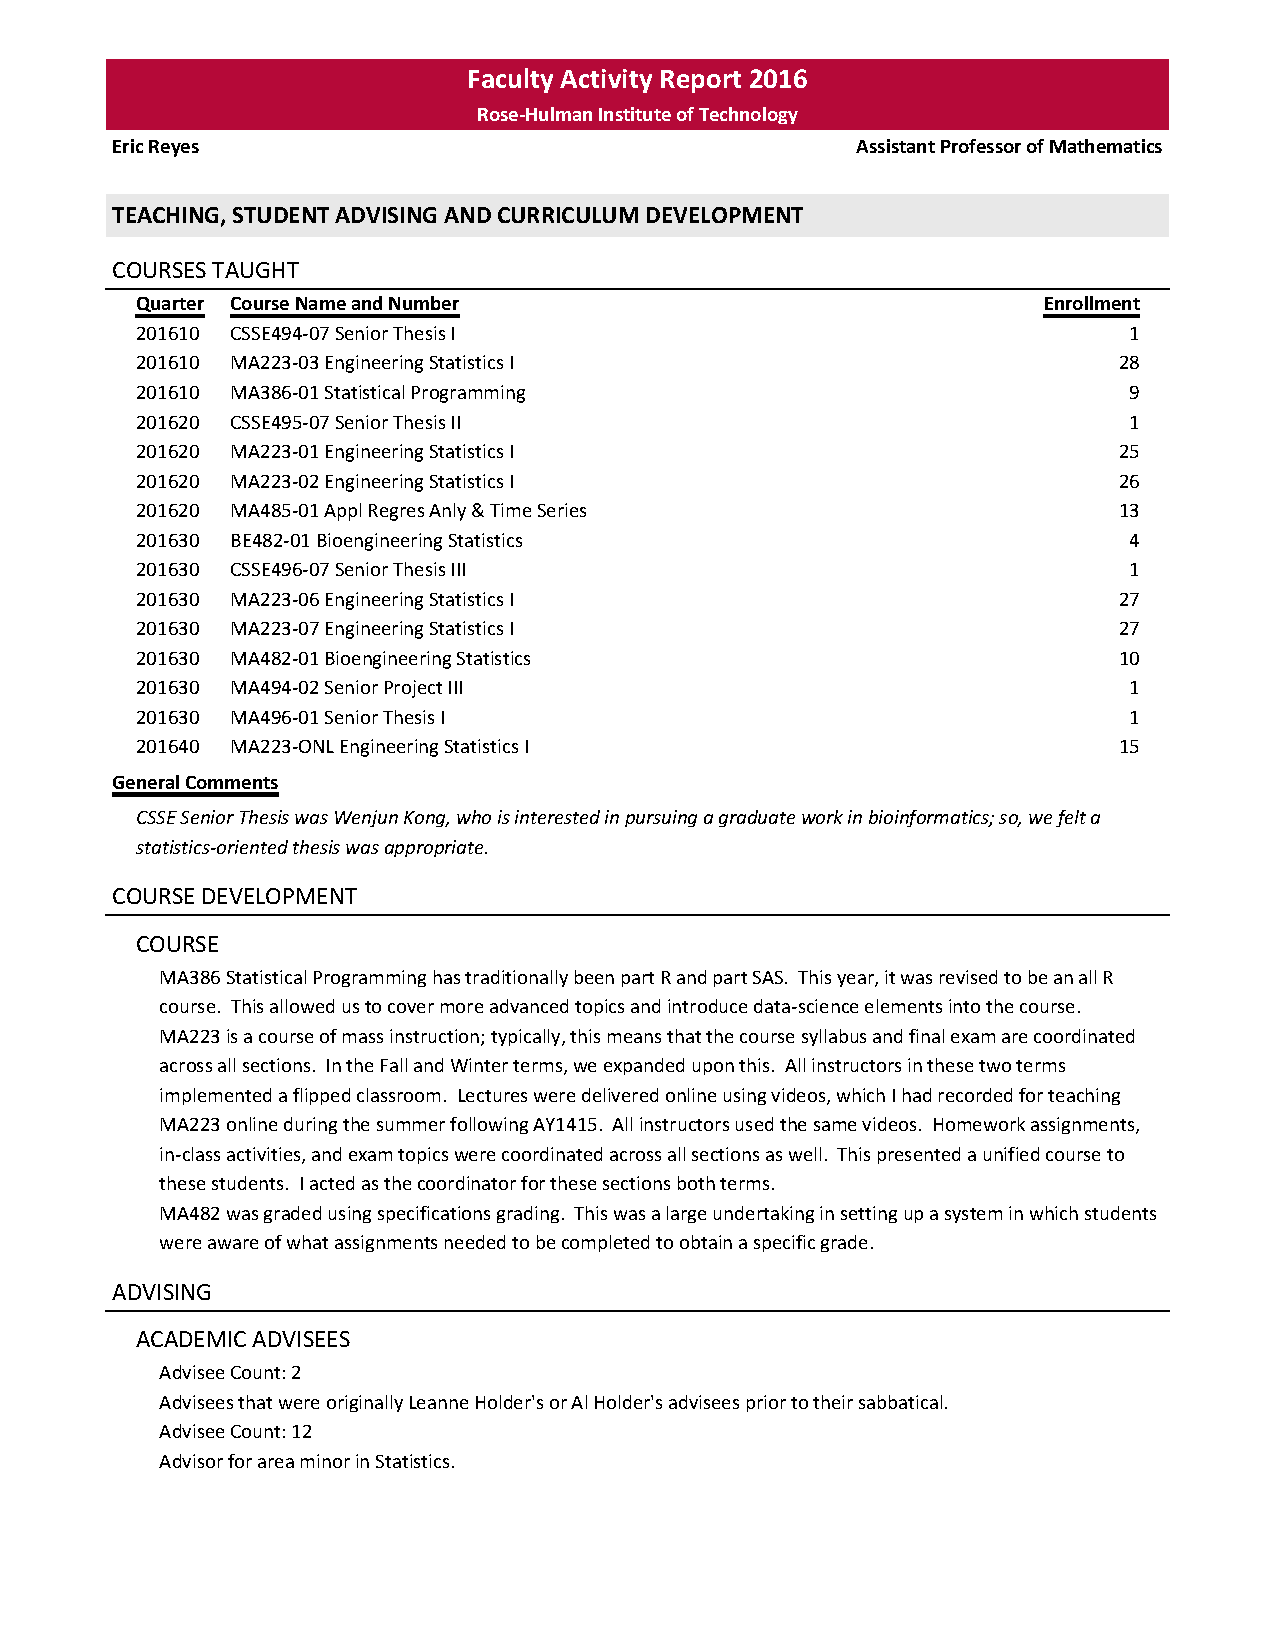
\includepdf[pages=1, link, linkname=ReyesFAR1516, pagecommand={\thispagestyle{empty}\phantomsection\addcontentsline{toc}{section}{Faculty Activity Report, AY1516}}]{supportingdocs/ReyesFAR1516}
\includepdf[pages=2-]{supportingdocs/ReyesFAR1516}

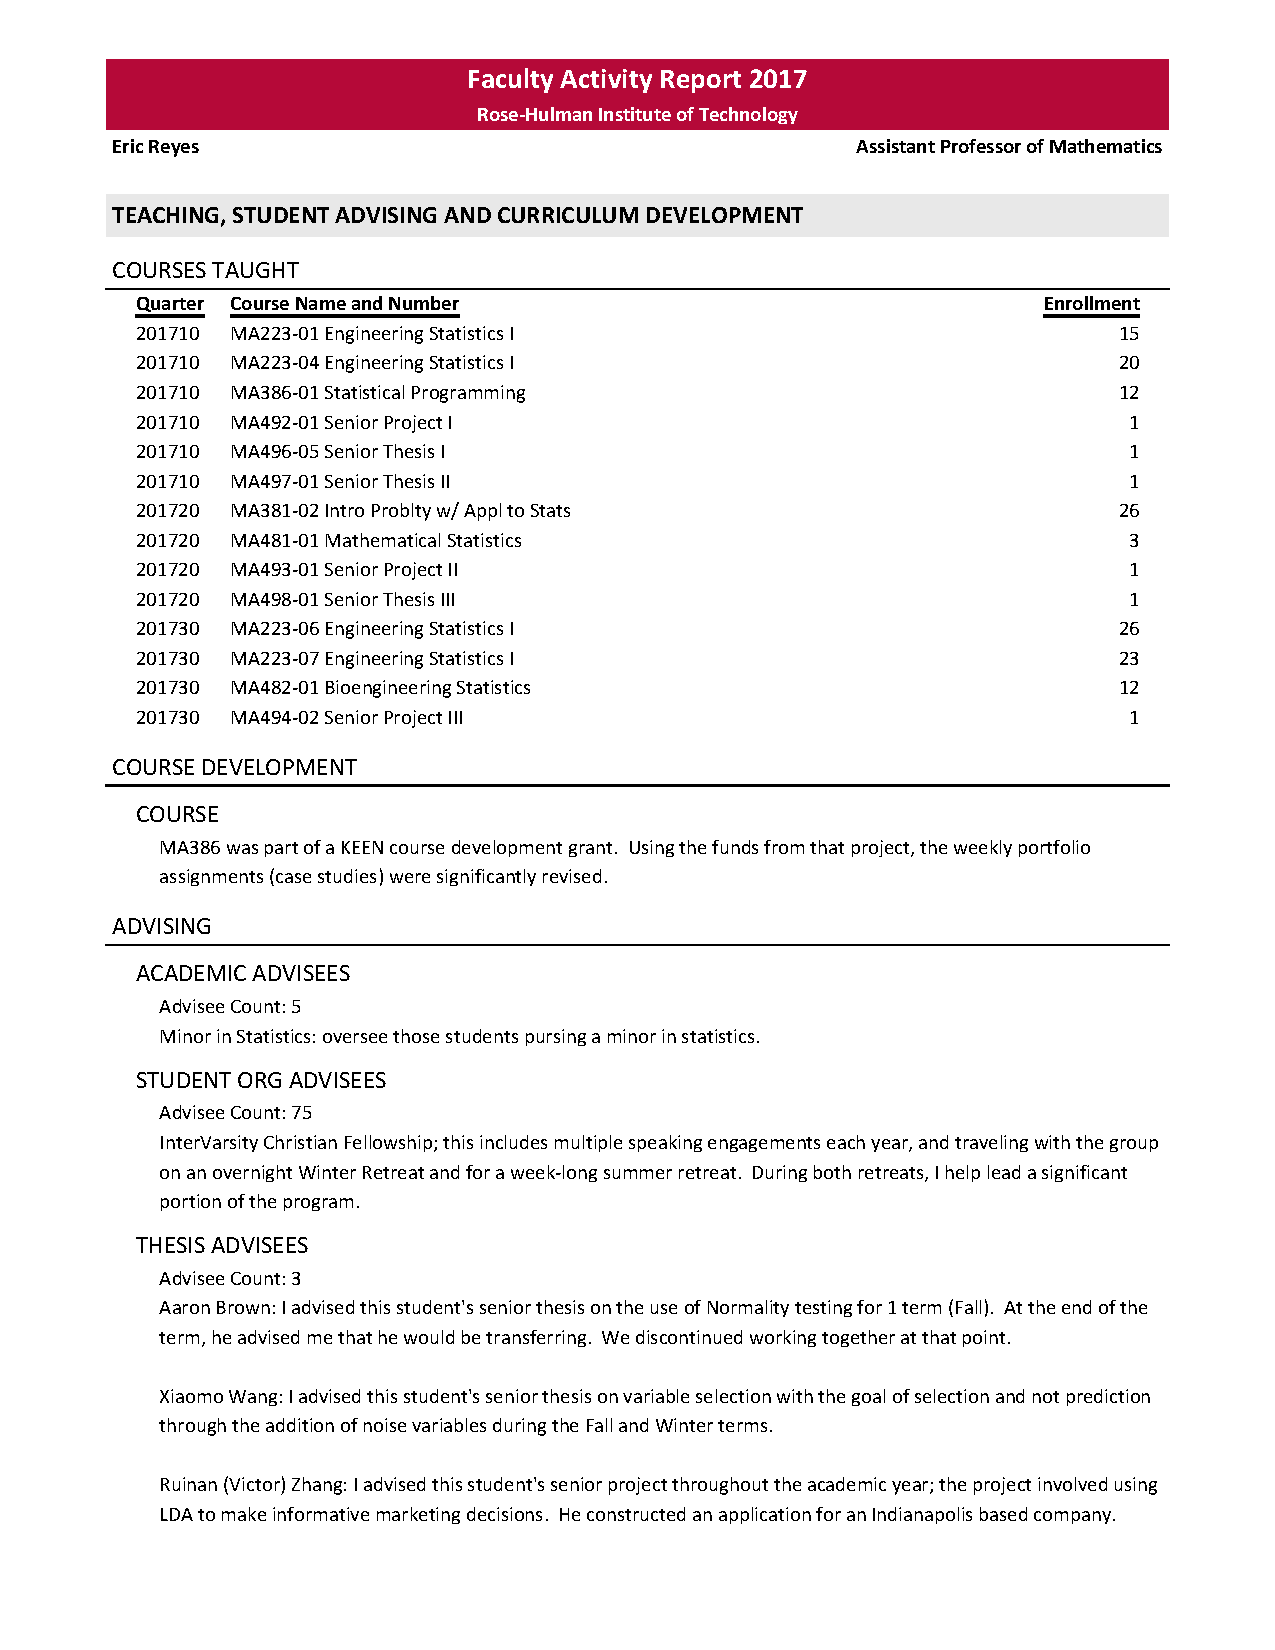
\includepdf[pages=1, link, linkname=ReyesFAR1617, pagecommand={\thispagestyle{empty}\phantomsection\addcontentsline{toc}{section}{Faculty Activity Report, AY1617}}]{supportingdocs/ReyesFAR1617}
\includepdf[pages=2-]{supportingdocs/ReyesFAR1617}

\includepdf[pages=1, link, linkname=ReyesFAR1718, pagecommand={\thispagestyle{empty}\phantomsection\addcontentsline{toc}{section}{Faculty Activity Report, AY1718}}]{supportingdocs/ReyesFAR1718}
\includepdf[pages=2-]{supportingdocs/ReyesFAR1718}

\includepdf[pages=1, link, linkname=ReyesFAR1819, pagecommand={\thispagestyle{empty}\phantomsection\addcontentsline{toc}{section}{Faculty Activity Report, AY1819}}]{supportingdocs/ReyesFAR1819}
\includepdf[pages=2-]{supportingdocs/ReyesFAR1819}

\includepdf[pages=1, link, linkname=ReyesFAR1920, pagecommand={\thispagestyle{empty}\phantomsection\addcontentsline{toc}{section}{Faculty Activity Report, AY1920}}]{supportingdocs/ReyesFAR1920}
\includepdf[pages=2-]{supportingdocs/ReyesFAR1920}

\includepdf[pages=1, link, linkname=ReyesFAR2021, pagecommand={\thispagestyle{empty}\phantomsection\addcontentsline{toc}{section}{Faculty Activity Report, AY2021}}]{supportingdocs/ReyesFAR2021}
\includepdf[pages=2-]{supportingdocs/ReyesFAR2021}

\includepdf[pages=1, link, linkname=ReyesFAR2122, pagecommand={\thispagestyle{empty}\phantomsection\addcontentsline{toc}{section}{Faculty Activity Report, AY2122}}]{supportingdocs/ReyesFAR2122}
\includepdf[pages=2-]{supportingdocs/ReyesFAR2122}

\includepdf[pages=1, link, linkname=ReyesFAR2223, pagecommand={\thispagestyle{empty}\phantomsection\addcontentsline{toc}{section}{Faculty Activity Report, AY2223}}]{supportingdocs/ReyesFAR2223}
\includepdf[pages=2-]{supportingdocs/ReyesFAR2223}

\includepdf[pages=1, link, linkname=ReyesFAR2324, pagecommand={\thispagestyle{empty}\phantomsection\addcontentsline{toc}{section}{Faculty Activity Report, AY2324}}]{supportingdocs/ReyesFAR2324}
\includepdf[pages=2-]{supportingdocs/ReyesFAR2324}

\chapter{Department Head Reviews}\label{department-head-reviews}

\includepdf[pages=1, link, linkname=DHReview1213, pagecommand={\thispagestyle{empty}\phantomsection\addcontentsline{toc}{section}{Dept. Head Review, AY1213}}]{supportingdocs/DHReview1213}
\includepdf[pages=2-]{supportingdocs/DHReview1213}

\includepdf[pages=1, link, linkname=DHReview1314, pagecommand={\thispagestyle{empty}\phantomsection\addcontentsline{toc}{section}{Dept. Head Review, AY1314}}]{supportingdocs/DHReview1314}
\includepdf[pages=2-]{supportingdocs/DHReview1314}


\includepdf[pages=1, link, linkname=DHReview1415, pagecommand={\thispagestyle{empty}\phantomsection\addcontentsline{toc}{section}{Dept. Head Review, AY1415}}]{supportingdocs/DHReview1415}

\includepdf[pages=2-]{supportingdocs/DHReview1415}


\includepdf[pages=1, link, linkname=DHReview1516, pagecommand={\thispagestyle{empty}\phantomsection\addcontentsline{toc}{section}{Dept. Head Review, AY1516}}]{supportingdocs/DHReview1516}

\includepdf[pages=2-]{supportingdocs/DHReview1516}

\includepdf[pages=1, link, linkname=DHReview1617, pagecommand={\thispagestyle{empty}\phantomsection\addcontentsline{toc}{section}{Dept. Head Review, AY1617}}]{supportingdocs/DHReview1617}
\includepdf[pages=2-]{supportingdocs/DHReview1617}

\includepdf[pages=1, link, linkname=DHReview1718, pagecommand={\thispagestyle{empty}\phantomsection\addcontentsline{toc}{section}{Dept. Head Review, AY1718}}]{supportingdocs/DHReview1718}
\includepdf[pages=2-]{supportingdocs/DHReview1718}

\includepdf[pages=1, link, linkname=DHReview1819, pagecommand={\thispagestyle{empty}\phantomsection\addcontentsline{toc}{section}{Dept. Head Review, AY1819}}]{supportingdocs/DHReview1819}
\includepdf[pages=2-]{supportingdocs/DHReview1819}

\includepdf[pages=1, link, linkname=DHReview1920, pagecommand={\thispagestyle{empty}\phantomsection\addcontentsline{toc}{section}{Dept. Head Review, AY1920}}]{supportingdocs/DHReview1920}
\includepdf[pages=2-]{supportingdocs/DHReview1920}

\includepdf[pages=1, link, linkname=DHReview2021, pagecommand={\thispagestyle{empty}\phantomsection\addcontentsline{toc}{section}{Dept. Head Review, AY2021}}]{supportingdocs/DHReview2021}
\includepdf[pages=2-]{supportingdocs/DHReview2021}

\includepdf[pages=1, link, linkname=DHReview2122, pagecommand={\thispagestyle{empty}\phantomsection\addcontentsline{toc}{section}{Dept. Head Review, AY2122}}]{supportingdocs/DHReview2122}
\includepdf[pages=2-]{supportingdocs/DHReview2122}

\includepdf[pages=1, link, linkname=DHReview2223, pagecommand={\thispagestyle{empty}\phantomsection\addcontentsline{toc}{section}{Dept. Head Review, AY2223}}]{supportingdocs/DHReview2223}
\includepdf[pages=2-]{supportingdocs/DHReview2223}

\includepdf[pages=1, link, linkname=DHReview2324, pagecommand={\thispagestyle{empty}\phantomsection\addcontentsline{toc}{section}{Dept. Head Review, AY2324}}]{supportingdocs/DHReview2324}
\includepdf[pages=2-]{supportingdocs/DHReview2324}



\end{document}
